\section{Overview}
<<<<<<< HEAD
\emph{Travlendar+} is an application that schedules the user's appointments, taking into account various tasks types, traffic information and so on. To do that as well as possible, the system is composed by four tiers, which are: the client layer, the web server layer, the application server layer and the data layer.
=======
\emph{Travlendar+} is an application that schedules the user's appointments, taking into account various tasks types, traffic information and so on. To do that as well as possible, the system is composed by four main tiers, that define the client layer, the web server layer, the application server layer and the data layer.
>>>>>>> ad258dd7c9a37861a484c05c0be22fc9761a519f

\emph{Travlendar+} uses these four layers to guarantee the best flexibility of the application, indeed the user can access to his calendar through either the web or the mobile application. Moreover, these four tiers permit to have a system that is easily maintained by developers.

\begin{figure}[H]
    \centering
    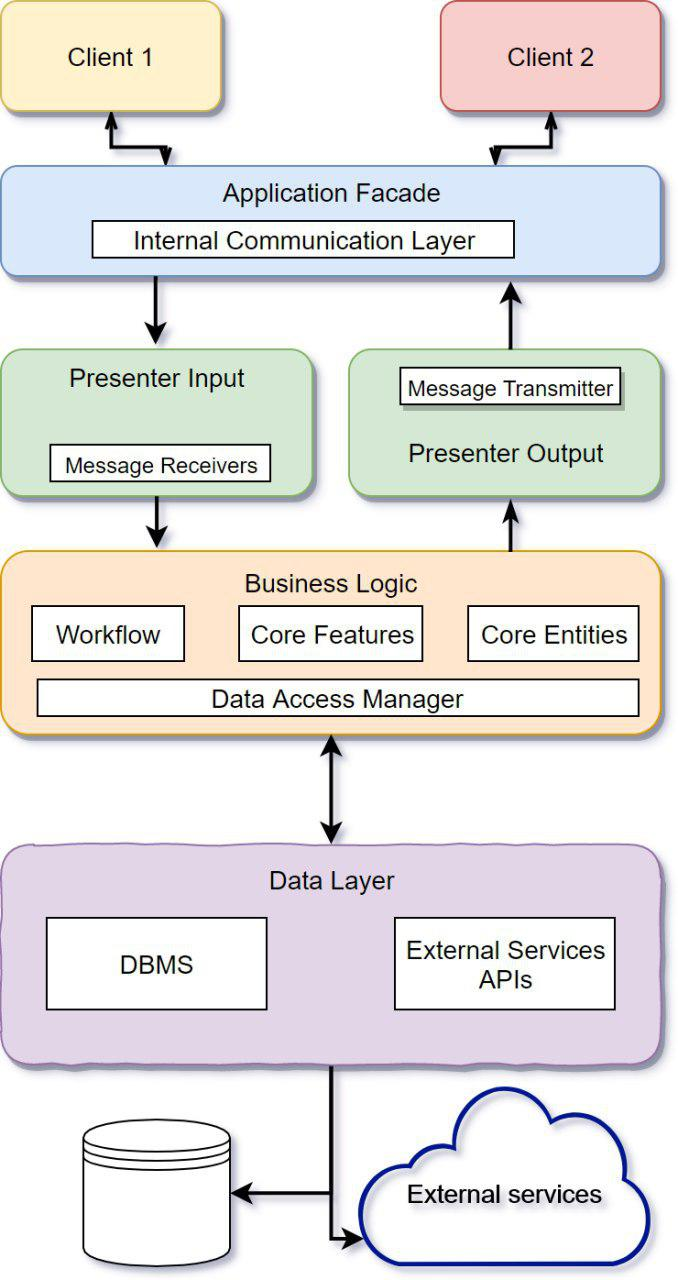
\includegraphics[scale=0.7]{Pictures/OverviewPictures/overviewDiagram.jpg}
    \caption{Overview of the \emph{Travlendar+} System}
\end{figure}

\begin{figure}[H]
    \centering
    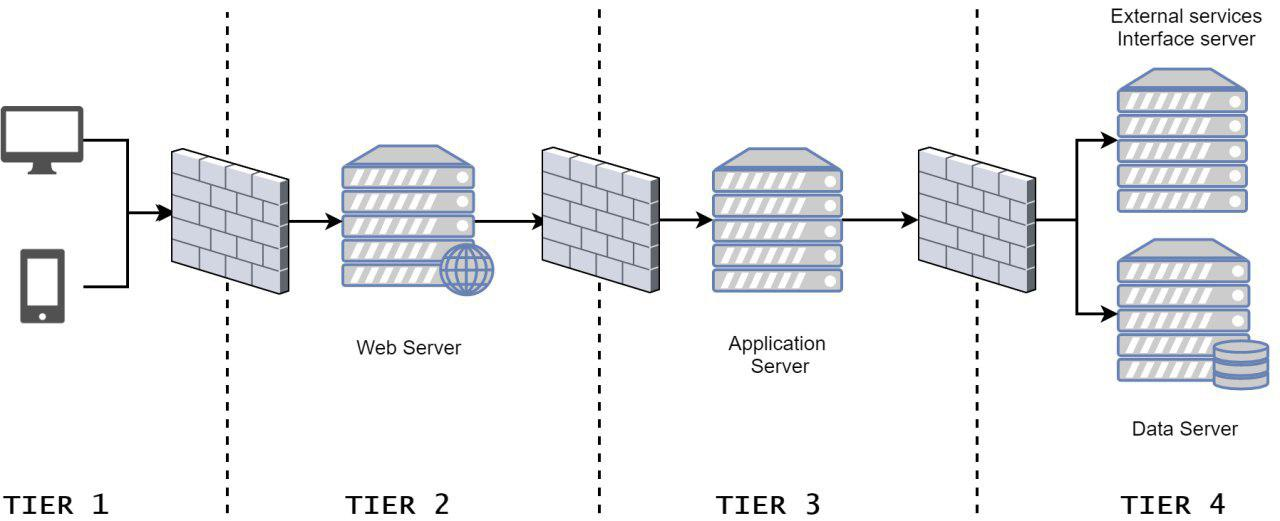
\includegraphics[scale=0.7]{Pictures/OverviewPictures/physical.jpg}
    \caption{Physical architecture of the \emph{Travlendar+} System}
\end{figure}

<<<<<<< HEAD
The application is divided into seven main components, the \emph{web client} and the \emph{mobile application client}, the \emph{Application Façade}, the \emph{Presenter Input} and the \emph{Presenter Output}, the \emph{Business Logic} and finally the \emph{Data Layer}.

When a client wants to connect to the application, through a web page (or a mobile application interface) sends an https request, according to the REST protocol. This request is received by the \emph{Travlendar+} web server, that contains the \emph{Application Façade} component. The web server is used in order to create a secure zone for the application server, in this way several hacks can be avoided. The web server takes the https request, translate it in a socket request and then send it to the application server, through the \emph{Presenter Input} component. This component is used to call the correct functionalities of the \emph{Business Logic}, that is the core of the entire system. This layer is used to add a new user to the system, to control the login system, to create a calendar, to add/modify/delete a task and to compute a travel. The \emph{Business Logic} component indeed does the required operations on the user datas, then interacts with the \emph{Data Layer} component to store these information or to receive some information either from the internal database or from an external service. For this reason the \emph{Data Layer} component is used to interact with both the internal DBMS and the external APIs services.

Finally, once the user's request is satisfied, the \emph{Business Logic} send the useful data to the \emph{Application Façade} component through the internal socket connection, provided by the \emph{Presenter Output} interface, and then the data are translated in a JSON file, and this is sent to the client.
=======
The application is divided into 7 main components, the \emph{web client} and the \emph{mobile application client}, the \emph{Application Façade}, the \emph{Presenter Input} and the \emph{Presenter Output}, the \emph{Business Logic} and finally the \emph{Data Layer}.

When a client wants to connect to the application, through a web page (or a mobile application interface) sends an https request, according to the REST protocol. This request is received by the \emph{Travlendar+} web server, that contains the \emph{Application Façade} component. The web server is used in order to create a secure zone for the application server, in this way several hacks can be avoided. The web server takes the https request, translate it in a socket request and then send it to the application server, through the \emph{Presenter Input} component. This component is used to call the correct functionalities of the \emph{Business Logic}, that is the core of the entire system. This layer is used to add a new user to the system, to control the login system, to create a calendar, to add/modify/delete a task and to compute a travel. The \emph{Business Logic} component so does the required operations on the user datas, then interacts with the \emph{Data Layer} component to store these information or to receive some information either from the internal database or from an external service. Indeed the \emph{Data Layer} component is used to interact with both the internal DBMS and the external APIs services.

Finally, once the user's request is satisfied, the \emph{Business Logic} send the useful datas to the \emph{Application Façade} component through the internal socket connection, provided by the \emph{Presenter Output} interface, and then the datas are translated in a JSON file, and this is sent to the client.
>>>>>>> ad258dd7c9a37861a484c05c0be22fc9761a519f
